%%
%% This is file `sample-manuscript.tex',
%% generated with the docstrip utility.
%%
%% The original source files were:
%%
%% samples.dtx  (with options: `manuscript')
%% 
%% IMPORTANT NOTICE:
%% 
%% For the copyright see the source file.
%% 
%% Any modified versions of this file must be renamed
%% with new filenames distinct from sample-manuscript.tex.
%% 
%% For distribution of the original source see the terms
%% for copying and modification in the file samples.dtx.
%% 
%% This generated file may be distributed as long as the
%% original source files, as listed above, are part of the
%% same distribution. (The sources need not necessarily be
%% in the same archive or directory.)
%%
%% The first command in your LaTeX source must be the \documentclass command.
%%%% Small single column format, used for CIE, CSUR, DTRAP, JACM, JDIQ, JEA, JERIC, JETC, PACMCGIT, TAAS, TACCESS, TACO, TALG, TALLIP (formerly TALIP), TCPS, TDSCI, TEAC, TECS, TELO, THRI, TIIS, TIOT, TISSEC, TIST, TKDD, TMIS, TOCE, TOCHI, TOCL, TOCS, TOCT, TODAES, TODS, TOIS, TOIT, TOMACS, TOMM (formerly TOMCCAP), TOMPECS, TOMS, TOPC, TOPLAS, TOPS, TOS, TOSEM, TOSN, TQC, TRETS, TSAS, TSC, TSLP, TWEB.
% \documentclass[acmsmall]{acmart}

%%%% Large single column format, used for IMWUT, JOCCH, PACMPL, POMACS, TAP, PACMHCI
% \documentclass[acmlarge,screen]{acmart}

%%%% Large double column format, used for TOG
% \documentclass[acmtog, authorversion]{acmart}

%%%% Generic manuscript mode, required for submission
%%%% and peer review
%\documentclass[manuscript,screen]{acmart}
\documentclass[sigconf, screen, review]{acmart}

%%
%% \BibTeX command to typeset BibTeX logo in the docs
\AtBeginDocument{%
  \providecommand\BibTeX{{%
    \normalfont B\kern-0.5em{\scshape i\kern-0.25em b}\kern-0.8em\TeX}}}

%% Rights management information.  This information is sent to you
%% when you complete the rights form.  These commands have SAMPLE
%% values in them; it is your responsibility as an author to replace
%% the commands and values with those provided to you when you
%% complete the rights form.
%\setcopyright{acmcopyright}
%\copyrightyear{2020}
%\acmYear{2020}
%\acmDOI{10.1145/1122445.1122456}

%% These commands are for a PROCEEDINGS abstract or paper.
%\acmConference[Woodstock '18]{Woodstock '18: ACM Symposium on Neural
 % Gaze Detection}{June 03--05, 2018}{Woodstock, NY}
%\acmBooktitle{Woodstock '18: ACM Symposium on Neural Gaze Detection,
 % June 03--05, 2018, Woodstock, NY}
%\acmPrice{15.00}
%\acmISBN{978-1-4503-XXXX-X/18/06}
\usepackage{booktabs}
\usepackage{bbding}
\usepackage{pifont}
\usepackage{wasysym}
\usepackage{amssymb}
\usepackage{tabularx}

\usepackage{todonotes}
\let\xtodo\todo
\renewcommand{\todo}[1]{\xtodo[inline]{#1}}
\newcommand{\itodo}[1]{\xtodo[inline]{#1}}
\newcommand{\todor}[1]{\textcolor{red}{#1}}
\newcommand{\insertref}[1]{\xtodo[color=green!40]{#1}}
\newcommand{\todos}[1]{\xtodo[inline,color=yellow!50]{Sven: #1}}
\newcommand{\todoj}[1]{\xtodo[inline,color=orange!50]{Jordan: #1}}
\newcommand{\todok}[1]{\xtodo[inline,color=green!50]{M and K: #1}}


\newcommand{\red}[1]{\textcolor{red}{#1}}

%%
%% end of the preamble, start of the body of the document source.
\begin{document}

%%
%% The "title" command has an optional parameter,
%% allowing the author to define a "short title" to be used in page headers.
\title{Revisiting Augmented Piano Prototypes: Does Augmentation Aid in Learning? }

%%
%% The "author" command and its associated commands are used to define
%% the authors and their affiliations.
%% Of note is the shared affiliation of the first two authors, and the
%% "authornote" and "authornotemark" commands
%% used to denote shared contribution to the research.
%\author{Jordan Aiko Deja}

%\orcid{1234-5678-9012}
%\affiliation{%
 % \institution{University of Primorska}
%  \city{Koper}
%  \country{Slovenia}
%  \postcode{6000}}
%\email{jordan.deja@famnit.upr.si}

%\author{Matjaž Kljun}
%\affiliation{%
%  \institution{University of Primorska}
 % \city{Koper}
 % \country{Slovenia}
%  \postcode{6000}}
%\email{matjaz.kljun@famnit.upr.si}

%\author{Klen Čopič Pucihar}
%\affiliation{%
%  \institution{University of Primorska}
% \city{Koper}
%  \country{Slovenia}
%  \postcode{6000}}
%\email{klen.copic@famnit.upr.si}

%%
%% By default, the full list of authors will be used in the page
%% headers. Often, this list is too long, and will overlap
%% other information printed in the page headers. This command allows
%% the author to define a more concise list
%% of authors' names for this purpose.
%\renewcommand{\shortauthors}{Deja, et al.}
%%
%% The abstract is a short summary of the work to be presented in the
%% article.
\begin{abstract}
Humans have been using and learning musical instruments for several centuries. In the recent two decades, innovations augmenting music instruments have been introduced to support learning of novice users and improvisation of performers. Of these innovations introduced, 49\% consists of augmented piano prototypes alone. Given this figure, there has not been a review done on these prototypes describing the different trends and approaches in augmenting the piano in relation to learning. In this paper, we present a systematic review of augmented piano prototypes in contrast to other augmented music instruments. We gathered and analyzed data from papers published within the last two decades that described an augmented piano prototype. Our findings present different contribution themes and their impact to piano design and learning. Lastly, we also present some recommendations and future directions on how to improve the piano learning process with the use of augmented technologies. 
\end{abstract}
%%
%% The code below is generated by the tool at http://dl.acm.org/ccs.cfm.
%% Please copy and paste the code instead of the example below.
%%
\begin{CCSXML}
<ccs2012>
    <concept>
        <concept_id>10010405.10010469.10010475</concept_id>
        <concept_desc>Applied computing~Sound and music computing</concept_desc>
        <concept_significance>500</concept_significance>
    </concept>
    <concept>
        <concept_id>10003120.10003121</concept_id>
        <concept_desc>Human-centered computing~Human computer interaction (HCI)</concept_desc>
        <concept_significance>500</concept_significance>
    </concept>
    <concept>
        <concept_id>10003120.10003121.10003125</concept_id>
        <concept_desc>Human-centered computing~Interaction devices</concept_desc>
        <concept_significance>500</concept_significance>
    </concept>
    <concept>
        <concept_id>10010405.10010489.10010491</concept_id>
        <concept_desc>Applied computing~Interactive learning environments</concept_desc>
        <concept_significance>300</concept_significance>
    </concept>
 </ccs2012>
\end{CCSXML}

\ccsdesc[500]{Human-centered computing~Human computer interaction (HCI)}
\ccsdesc[500]{Human-centered computing~Interaction devices}
\ccsdesc[300]{Applied computing~Sound and music computing}
\ccsdesc[300]{Applied computing~Interactive learning environments}
%%
%% Keywords. The author(s) should pick words that accurately describe
%% the work being presented. Separate the keywords with commas.
\keywords{augmented piano, music learning, systematic review, survey, piano}
%%
%% This command processes the author and affiliation and title
%% information and builds the first part of the formatted document.
\maketitle
\todok{Please give feedback. Thank you!}
\section{Introduction}
%%%
%% This paragraph gives a high level introduction into the topic, how music instruments evolved and why it is hard to learn them. 
%%%
In the past 500 years, acoustic musical instruments have matured from simple, less complex instruments into the huge variety of instruments we know today. At the same time, today's instruments allow to generate a larger variety of sounds making learning an instrument more sophisticated. Thus, today playing a musical instrument is a well respected profession which requires a high level of perseverance and discipline. As acquiring the skills required to play an instrument is hard and takes time, humans have been designing innovations improving the experiences of learning and playing these musical instruments. Just within this century, we have observed and seen several technology interventions being introduced to improve musical instruments. These innovations have transformed acoustic instruments into what we now know as digital instruments \cite{magnusson2007acoustic}. Digital instruments recreate their acoustic counterparts offering exclusive benefits that were not seen in acoustic devices such as portability, having no need for tuning and having immunity to harmful conditions like humidity. In addition, digital music instruments provide users with recording capabilities, volume controls, and headphone jacks for sound privacy without disturbing people around them. 
%%%
%% This paragraph highlights how learning has been done in the past.
%%%
Learning an instrument has a long tradition in almost every culture, and the process does not differ widely between societies. Here, the very traditional way is that an experienced musician, the teacher, is passing on the knowledge to a novice, the student. Normally these sessions with the teacher and student are complimented by personal practice, acquiring the skills needed for the next session with a teacher. This method is not only true for learning a new instrument but also often for new languages. In the domain of learning new languages, we already have successful alternatives using computer-supported learning lessons, often fully replacing the teacher role using learning apps such as Duolingo\footnote{\url{https://duolingo.com/}}. While reading musical notes can be acquired in a similar matter, musical instruments are fundamentally different as there is a physical element to it - the art of producing a sound. However, researchers argue that by augmenting the musical instrument itself, guidance can be provided to the novice directly on and around the physical musical instrument. Just in the recent two decades, augmentations have been introduced to help novices in this process. String instruments like the violin \cite{overholt2005overtone}, woodwind instruments (e.g. clarinet \cite{silva2008interaction}), pianos \cite{mcpherson2010augmenting} and other instrument classes \cite{turchet2018some, newton2011examining} have been equipped with auxiliary hardware, peripherals, and sensors to improve sound quality, or track user motion while playing these instruments. Software features in the form of learning modules have also been introduced in these instruments. These allowed novices to practice on their own \cite{fober2007vemus}, interact with a virtual agent \cite{costalonga2008agent, tidemann2009groovy}, and read complex notation easily with the help of overlaid visualizations \cite{trujano2018arpiano, gerry2019adept, santiniaugmented}. These augmentations also introduced newer affordances that play an important role in learning \cite{dede1996evolution}. Therefore, it is important to study how learning a musical instrument augmented with digital technology improves the learning experience.
%%%
%% This paragraph should now focus on pianos only and how augmenting a piano can improve the learning. 
%%%
The acoustic piano has been a popular choice by early stage musicians (7 out 10 had the piano as the first instrument they learned during their musical career \cite{sloboda1992transitions}, which ranks second to the violin). Several socio-cultural, personal skill benefits and improvements have been attributed as well with adult piano users \cite{jutras2006benefits}. In terms of ergonomics, pianists and violinists share their own difficulties especially with prolonged usage and practice \cite{chi2020ergonomics}. Adaptive accessories such as chin and/or shoulder rests have been proposed to improve the interface between the instrument and the player. However, the case does not remain the same for pianists. The piano's physical features, following a one-size-fits-all layout, have been a long recognized-industry standard, yet this has been observed to discriminate against many pianists, novices, even female players \cite{boyle2012experience}. This is just one of the many reasons why researchers have focused heavily on piano augmentation. To elaborate, using an acoustic piano would involve fixing your posture while at the same time ensuring proper positioning of the fingers on the keys. Learners have to consider this for both hands and at the same time have to consider timing of and coordination with the foot on the pedals. For most novice learners, getting used to these motor skills along with reading and memorizing complex music sheet notation can be very overwhelming which makes learning even more difficult \cite{highben2004effects}. 
%%i made a suggested improvement of this paragraph. see the one above it
%Due to the piano's physical layout and the complexity to master the instrument, researchers  focused heavily on piano augmentation. For example, using an acoustic piano would involve fixing your posture, proper positioning of the fingers on the keys and feet on the pedals. In using a digital keyboard, users also need to setup power supply of the device, connection to a computer and other peripherals (when recording) and enabling or disabling specific modes such as practice modes with lighted keys that guide users in key press, a playback mechanism and other features of its digital interface. It is important to note that these innovations changed how experienced users play these instruments (in terms of self expression, music recording and sharing), but may have not necessarily-aided in the learning process of novice users \cite{bown2009understanding}. This has opened newer avenues and opportunities to augment the piano with the novice user as the main focus. Thus, in the following investigation we will primarily investigate piano augmentations.  
%%% 
%% This paragraph now flashes out the paper - with a particular focus on the contribution.
%%%
Due to the large number of presented augmented piano prototypes over the last years in various fields, the goal of this paper is to understand the general space, challenges as well as opportunities for piano augmentation. Thus, we first present a literature review on piano augmentation with a special focus on augmentation for an enhanced learning experience. Based on our literature review of sixty one (61) papers, we first present the current state-of-the-art of piano augmentation and then present future directions for augmented piano. Finally, we provide recommendations based on our discussion and relevant existing frameworks with the ultimate goal of augmenting the ideal piano prototype towards supporting several stages of piano learning. 
%As a first goal, this paper aims to review the different types of augmentations done on the piano. These contributions will be analyzed based on the type of augmentation and how this improves the piano learning experience for the novice user. We did a literature scan on digital libraries and repositories and we found out that augmented piano prototypes form a great number of papers published compared to other augmented musical instruments (such as the guitar, drum, flute, violin and many others). These augmentations and contributions have been designed with varying contexts in mind. As such, replicating these studies will depend on various factors such as accessibility of required hardware, difficulty of recreating assets, available open-source libraries and willing participants for user studies. Thus, as a second goal, we intend to guide our readers on future directions in introducing novel contributions in the augmented piano. We shall do this by summarizing and organizing these state-of-the-art contributions into categories. Then, we shall provide recommendations based on our discussion and relevant existing frameworks that support learning. 
%different trends and categories that have improved AR experiences with special emphasis to the piano. Even though there have been several augmented piano prototypes in current literature, we believe that only a few are developed with focus on improving how piano novices learn (and towards having sustainable, meaningful learning experiences). The different novel contributions in piano AR have been measured to be effective based on several metrics such as registration speed, quality of graphics, and observed learner performance. These studies have been written with a distinct context in mind. As such, replicating these studies will depend on various factors such as: accessibility of required hardware, difficulty of recreating assets, available open-source libraries and willing participants for user studies. As a second goal, we intend to guide researchers on possible directions towards introducing novel contributions in augmented piano prototypes. We shall do this by summarizing the state-of-the-art implementation and evaluation of included literature. Then, we enumerate recommendations for learning piano with AR and discuss relevant innovations and models that can support these recommendations.
%The paper is organized as follows: Section \ref{sec: bg} provides the basics on piano learning and our definition of augmentation. Section \ref{sec: method} describes our methods for qualitative analysis. Section \ref{sec: trends} discusses the results of our analysis of the trends in augmented piano prototypes designed throughout the years. These include state-of-the-art contributions (in the design, engineering and content). We organise these strategies into categories such as hardware and peripheral, user interface modes and audio-visual projections that support learning (such as hand tracking, visualisations, agents and tutors) and discuss each of them in Section \ref{sec: strat}. Lastly, Section \ref{sec: discuss} concludes this paper with our recommendation for future augmented piano prototypes. 
%One of these innovations is through Augmented Reality (AR). The earliest known prototype designed with AR came in the late 90s in the form of a musical keyboard display with keyboard input method \cite{breitweiser1996musical}. This along with other AR prototypes rode the waves of the Information era, with the boom of the World Wide Web, the emergence of the millennium bug, higher resolution graphics, stronger processors and better tracking algorithms among many others. Since then, as several augmented piano prototypes have been developed, key innovations have shifted focus as well jumping from one technology to other (e.g. overlaying graphics to optimization to teaching modes). As these innovations shift focus from one to the other, human experiences are also reshaped by these changes. 
%This introduction is not yet done. I need to elaborate the second and third question in the abstract. 
%put this somewhere
%Several technologies have enabled the creation of hardware, learning modes and interactive spaces. Over the last 20 years, we have observed progress in hardware computing power, tracking of elements in real-time (such has hand, object tracking) and in authoring AR tools, plug-ins and applications. These technologies are already seen and applied in several settings such as in tourism \cite{kounavis2012enhancing}, learning \cite{santos2013augmented}, manufacturing \cite{thomas1992augmented}, pilot training \cite{macchiarella2004augmented} and many others.
\todok{Please give feedback. Thank you!}
\section{On Music Learning}
When learning music and how to play musical instruments, different methodologies and instructional settings are usually considered. There are four major methodologies that formal institutions integrate in their techniques when teaching music and instruments. %These are (1) Kodály method \cite{choksy1974kodaly}, (2) Orff Schulwerk \cite{shamrock1997orff}, simply referred to as the Orff approach, (3) Dalcroze eurhythmics \cite{mead1994dalcroze} and the (4) Suzuki method \cite{peak1998suzuki}.
(1)~The Kodály method \cite{choksy1974kodaly} aims its learners to have a solid grasp of music theory and music notation on both verbal and written forms. In this technique, hand signals, referred to as \textit{solfège}, along with musical shorthand notation, and rhythm verbalization are used to teach children learners. (2) The Orff Schulwerk \cite{shamrock1997orff} approach tackles its pupils with the rudimentary forms of music at an early stage. The Orff approach considers the body as a percussive instrument, as such it fosters self-discovery and improvisation which moves far away from repetitive mechanical drills. (3) The Dalcroze method \cite{mead1994dalcroze} is considered as the rhythm gymnastics approach to music learning. Novices are instructed to emphasize physical awareness and engage with music involving all their senses and even kinesthetic skills. (4) The Suzuki method \cite{peak1998suzuki} draws inspiration in music learning similar to the approaches of learning one's native language. It describes an ideal environment that considers, high-quality music samples, rote (mechanical) training and repetition. Apart from these four internationally-renown methods, there are other approaches that have been influential to music learning as well. 

In addition, the music learning process considers several domains such as the psychomotor domain, the cognitive domain, and the affective domain of its learners. The psychomotor domain in music education focuses on the development of skills of the learner in relation to visual, auditory and tactile perception \cite{simpson1966classification} and the movements and responses that the body performs from these stimuli. The cognitive domain in music learning describes the process of how a learner acquires knowledge of important concepts and foundations in music. Understanding how the learner acquires, retains and applies knowledge in the music learning process is considered a strategic approach that leads to more effective music learning experience \cite{hanna2007new}. This domain works well with the different phases of music making such as performing, improvising, composing, arranging and even conducting. As these activities may require precise cognitive processing, having a concrete foundation of these procedural skills ensures proper development for the learner \cite{westerlund2003reconsidering}. The affective domain considers the willingness of the learner to receive, reflect and share what they have acquired during the music learning process. This domain also considers music appreciation and sensitivity as response to the emergence of music education as an aesthetic learning process \cite{mccarthy2002music}. Here, learners use music with their feelings (thus the term affective) and are evoked into aesthetic experiences. 

Most of these approaches to learning music and music instruments have helped both learners and teachers deliver their instruction more effectively \cite{burns2020using}. In fact, some of these have inspired instrument augmentation as well \cite{howard1996kodaly, burns2020using, blackshaw2020wearing, anggoro2020study, comeau2012playing} which proves that their approaches can be applied in technology instrumentation. While it is not clear whether any of these approaches are more superior over the other, instrument especially piano augmentation can definitely draw inspiration from these approaches. True enough, the process of integrating these music teaching approaches with instrument technology augmentation has been documented to be trivial and subject to more improvement \cite{beckstead2001will}. 
%\subsection{Augmented Reality Piano Prototypes}
%Augmented Reality
%Augmented reality piano teaching systems
%Design Factors affecting augmented reality piano teaching systems (hardware, software, content)
\todok{Please give feedback. Thank you!}
\section{Method}
To understand the space of augmented pianos, in the following, we present a literature review following the \textit{Preferred Reporting Items for Systematic Reviews and Meta-Analyses} (\textbf{PRISMA}) technique \cite{moher2009preferred}. This paper performs a review of prototypes with learning as a focus, where we also subscribed to the techniques in the works of \cite{santos2013augmented, schneegass2016mobile, kljun2015transference, blattgerste2019augmented, mcpherson2015buttons, delgado2011state}. This guided us further on how to analyse and review these augmented piano prototypes for this specific context. The approach included a qualitative-analysis phase that discuses these innovations in the context of learning and the theme of augmentation. The steps performed in this systematic review is as follows: 

\subsection{Search for Prototypes}
%\label{subsec: search}
We did a literature search between March to October 2020 in several digital libraries such as Google Scholar, ACM Digital Library and IEEE Xplore Digital Library. As search terms, we used all combination of the following three keywords \{\texttt{"augmented reality", "AR", "augmented"}\} in combination with \{\texttt{"piano", "keyboard", "guitar", "drum", "violin", "flute"}\}. In a first round of search, we included other instruments in order to have a general understanding of piano and how many contributions are out there in contrast to other instruments. Resulting in search terms such as \{\texttt{"augmented reality piano"}\}. We included only scientific articles written in English. We found a total of 1,206 articles from our initial search terms across these digital libraries. It is important to note that some papers will appear in searches from at least two libraries and as such we have to note of these duplicates. Not filtering these, there were 595 articles on piano and keyboard (49.3\% of the results), 237 on violin (19.7\% of the results), 187 on guitar (15.5\% of the results), 156 on drum (12.9\% of the results), and 31 on flute (2.6\% of the results). 

\subsection{Inclusion Criteria}
%\label{subsec: criteria}
Since the focus of this survey is on augmented piano prototypes and in relation with piano learning, we filtered these papers based on a specific inclusion criteria. This is described below: 
\begin{enumerate}
    \item The paper discusses a piano
    \item The prototype is meant for playing, learning, or teaching the piano
    \item The prototype is an augmented piano 
\end{enumerate}
The authors classified all 1,206 initial papers based on the above criteria, filtering duplicates, which resulted in a selection of 61 articles. These papers discussed the design and evaluation of augmented piano prototypes. 

\subsection{Qualitative Analysis}
The final 61 papers which we identified using the structured literature review as described above served as the corpus for an in depth analysis of augmented piano prototypes. We designed the review to easily recognize common trends among the papers. Note that the goal is not to correctly describe which prototype is an augmented piano or not, but rather to gather enough examples of pianos that have been effectively-augmented towards playing or learning the piano.  In a next step, we classified the gathered literature by identifying them by themes, intent, and type of augmentation. These results will be presented and discussed in the following sections. 
%\subsection{Data Gathering}
%\label{subsec: gathering}
%A form was drafted to facilitate the gathering of data from the 61 included articles. The form seeks to retrieve the following information: (1) publication details, (2) contributions, (3) type of augmentation, (4) citation count, and (5) design and results of the user study.
%The publication details include the title of the paper, year of publication, authors etc. The contributions of each paper were extracted and analyzed as well. The use of augmentation refers to the set of features that were added into the piano - either hardware, software, or both. The design and results of the user study refer to the description of applicable user studies and tests. Other features include sample size, method, questionnaire, and tools used to conduct the user tests.
This is described below:(1)  The paper discusses a piano(2)The prototype is meant for playing, learning, or teachingthe piano(3)  The prototype is an augmented pian\section{Findings}

\subsection{Technology trends in augmentation}
%\label{sec: trends}
%\subsection{Trends in Non-AR augmented Piano Prototypes}

\begin{figure*}[t]
    \centering
    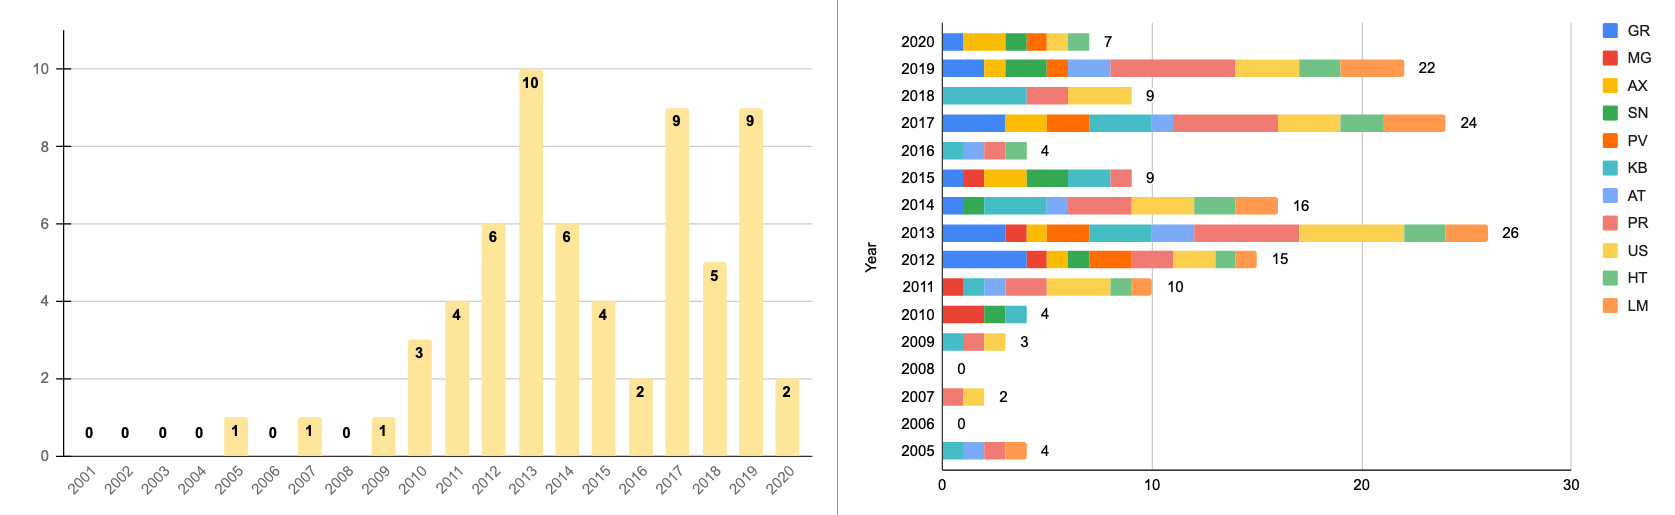
\includegraphics[width=18cm]{figures/yeartrend.png}
    \caption{\textbf{Left:} The distribution of the 61 augmented piano papers over the last two decades included in our literature review.  \textbf{Right:} Technology trends of augmented piano. A paper may have presented several technology augmentations as a contribution. 
    }
    \label{fig:doublechart}
\end{figure*}  
% reserved caption \textbf{Right:} Trend of contribution categories on the AR piano papers published within the last two decades. We have used moving average values to visualize the trends in these different contribution categories. 

\begin{table*}[h]
\caption{The corpus of the augmented piano papers and their features sorted in chronological order. Legend: \textit{\#} = number of citations; \textit{GR} = Gesture Recognition and optical scanners; \textit{MG} = magnets and resonators; \textit{AX} = other auxiliary hardware and peripherals attached; \textit{SN} = synthesizers ; \textit{PV}= projections and visualizations; \textit{KB} = AR keyboard; \textit{AT} = AR agents and tutors; \textit{PR} = piano roll and other visuals that simplify chords and notes; \textit{US} = user study; \textit{HT} = hand tracking; \textit{LM} = learning modes.}
\label{tab:overview}
\resizebox{\textwidth}{!}{%
\begin{tabular}{lllr|c|c|c|c|c|c|c|c|c|c|c|l} \toprule
\textbf{Paper} & \textbf{Author(s)}        & \textbf{Year} & \textbf{\#} & \textbf{GR} & \textbf{MG} & \textbf{AX} & \textbf{SN} & \textbf{PV}  & \textbf{KB} & \textbf{AT} & \textbf{PR} & \textbf{US} & \textbf{HT} & \textbf{LM} &  \textbf{more info} \\ \midrule
P01 & \citet{barakonyi2005augmented}      & 2005 & 47         & &&&&& \ding{51} & \ding{51} & \ding{51} &           &           & \ding{51} & \\ \hline
P02   & \citet{schmalstieg2007experiences}  & 2007 & 268        & &&&&&          &           & \ding{51} & \ding{51} &           &           & \\ \hline
P03 & \citet{correa2009computer}          & 2009 & 63         & &&&&& \ding{51} &           & \ding{51} & \ding{51} &           &           & \textit{patients w/ cerebral palsy}\\ \hline
P04 & \citet{mcpherson2010toward}           & 2010  &  3  &             & \ding{51} &            &             &  &      &&&&&&  \\ \hline
P05  & \citet{mcpherson2010augmenting}       & 2010 &  52  &            & \ding{51} &            & \ding{51} &                             &      &&&&&& \textit{synthesized sound blends with acoustic sound} \\ \hline
P06   & \citet{zhang2010affordable}         & 2010 & 22         & &&&&& \ding{51} &           &           &           &           &           & \\ \hline 
P07  & \citet{mcpherson2011multidimensional} & 2011  &  28  &            & \ding{51} &            &             &             &       &&& \ding{51} &&& \\ \hline
P08    & \citet{huang2011piano}              & 2011 & 50         & &&&&&  \ding{51} &           &           &           & \ding{51} &           & \\ \hline
P09   & \citet{xiao2010mirrorfugue}         & 2011 & 31         & &&&&&          & \ding{51} & \ding{51} & \ding{51} &           &           & \textit{3 unique interfaces}\\ \hline
P10   &  \citet{xiao2011duet}               & 2011 & 7          &  &&&&&          &           & \ding{51} & \ding{51} &           & \ding{51} & \textit{practice modes}\\ \hline 
P11  & \citet{hadjakos2012pianist}           & 2012  &  40 & \ding{51} &         &            &             &   \ding{51} &     &&&& \ding{51} &&   \\ \hline
P12  & \citet{nicolls2012gesturally}         & 2012  &  12  & \ding{51} &         & \ding{51} &  \ding{51}  &            &      &&&&&&  \\ \hline
P13  & \citet{yang2012augmented}             & 2012 &  20  & \ding{51} &         &            &             & \ding{51}  &      && \ding{51} &&&&   \\ \hline
P14  & \citet{p2012problem}                  & 2012 &  38  & \ding{51} & \ding{51} &            &             &    &      &&& \ding{51} &&& \textit{tests during several demos in universities, conservatories, etc} \\ \hline
P15   & \citet{takegawa2012piano}           & 2012 & 26         &  &&&&&         &           & \ding{51} & \ding{51} &           & \ding{51} & \\ \hline 
P16  & \citet{mcpherson2013space}            & 2013  &  16  & \ding{51} &         &  \ding{51}  &             &             &       &&&  \ding{51} &&& \textit{oscillatory motion finger tracking} \\ \hline
P17 & \citet{yang2013visual}                & 2013  &  5 & \ding{51} &         &            &             & \ding{51}  &      && \ding{51} &&&& \textit{even hanve Harp and Flock mode as type} \\ \hline
P18 & \citet{mcpherson2013portable}         & 2013  &  21  & \ding{51}  & \ding{51} &            &             & \ding{51} &     &&&&&& \textit{RGB LED lights as form of feedback and to aid in tracking}  \\ \hline
P19    & \citet{chow2013music}               & 2013 & 45         & &&&&& \ding{51} &           & \ding{51} & \ding{51} &           & \ding{51} & \\ \hline
P20    & \citet{weing2013piano}              & 2013 & 29         & &&&&&          &           & \ding{51} & \ding{51} & \ding{51} & \ding{51} & \textit{they used visualizations in a gamified approach}\\ \hline
P21    & \citet{chouvatut2013virtual}        & 2013 & 8          & &&&&& \ding{51} &           & \ding{51} &           &           &           & \textit{supports the rehabilitation of PWD's}\\ \hline
P22   & \citet{oka2013marker}               & 2013 & 27         &  &&&&&         &           &           &           & \ding{51} &           & \textit{piano fingering}\\ \hline
P23   & \citet{xiao2013mirrorfugue}         & 2013 & 17         &  &&&&&         & \ding{51} &           & \ding{51} &           &           & \\ \hline
P24   & \citet{leonard2013virtual}          & 2013 & 9          & &&&&& \ding{51} &           &           & \ding{51} &           &           & \\ \hline 
P25   & \citet{goodwin2013key}              & 2013 & 10         &  &&&&&         & \ding{51} & \ding{51} &           &           &           & \\ \hline
P26  & \citet{zandt2014piaf}                 & 2014 &  9 & \ding{51} &         &            & \ding{51} & &     &&&& \ding{51} && \textit{users gesture and augments equivalent sound of gesture}   \\ \hline
P27    & \citet{nugraha2014pemanfaatan}      & 2014 & 38         & &&&&& \ding{51} &           &           & \ding{51} &           &           & \\ \hline
P28   & \citet{xiao2014andante}             & 2014 & 28         &   &&&&&         & \ding{51} & \ding{51} &           &           & \ding{51} & \\ \hline 
P29   & \citet{raymaekers2014game}          & 2014 & 14         &  &&&&&         &           & \ding{51} & \ding{51} &           & \ding{51} & \textit{shooting game}\\ \hline
P30   & \citet{de2014infrared}              & 2014 & 6          & &&&&&\ding{51} &           &           &           & \ding{51} &           & \textit{magnetic glove}\\ \hline
P31   & \citet{kim2014ar}                   & 2014 & 11         & &&&&& \ding{51} &           & \ding{51} & \ding{51} &           &           & \\ \hline
P32 & \citet{fontana2015designing}          & 2015  &  3  &             & \ding{51} & \ding{51} & \ding{51} &                             &      &&&&&&  \\ \hline
P33  & \citet{chiang2015oncall}              & 2015  & 2   & \ding{51} &         &            &             &     & \ding{51} && \ding{51} &&&& \\ \hline
P34 & \citet{dahlstedt2015mapping}          & 2015  &  3  &             &         & \ding{51} &  \ding{51} &                             &      &&&&&& \textit{gravity models to track movement; synthesizes acoustic sound}  \\ \hline
P35   & \citet{zaqout2015augmented}         & 2015 & 1          & &&&&& \ding{51} &           &           &           &           &           & \\ \hline 
P36    & \citet{fernandez2016piano}          & 2016 & 7          &  &&&&&         & \ding{51} & \ding{51} &           &           &           & \\ \hline
P37   &  \citet{liang2016barehanded}        & 2016 & 20         & &&&&& \ding{51} &           &           &           & \ding{51} &           & \\ \hline
P38 & \citet{ogata2017keyboard}             & 2017  &  1  &  \ding{51}  &         &            &             &  \ding{51}  &       &&& \ding{51} & \ding{51} && \textit{motion tracking enhancing performance; shape distortion} \\ \hline
P39  & \citet{mcpherson20172012}             & 2017  &  41 &   \ding{51} &         &  \ding{51} &             &             &       &&&&&& \textit{surface coating and capacitive sensing} \\ \hline
P40 & \citet{liang2017piano}                & 2017  & 6 & \ding{51} &         & \ding{51} &             &  \ding{51} &     &&&&&& \textit{foot pedal as auxiliary hardware}  \\ \hline
P41    & \citet{hackl2017holokeys}           & 2017 & 7          & &&&&& \ding{51} &           & \ding{51} &           &           &           & \\ \hline
P42    & \citet{das2017music}                & 2017 & 5          & &&&&& \ding{51} & \ding{51} & \ding{51} &           &           & \ding{51} & \textit{has a lesson builder module independent of other modes} \\ \hline
P43   &  \citet{claudia2017yousician}       & 2017 & 0          & &&&&&           &           & \ding{51} &           &           &           & \\ \hline
P44   & \citet{kerdvibulvech2017innovative} & 2017 & 4          &  &&&&&\ding{51} &           &           & \ding{51} & \ding{51} &           & \textit{users gesture on air like piano air keys}\\ \hline
P45   & \citet{rogers2014piano}             & 2017 & 42         &   &&&&&        &           & \ding{51} & \ding{51} &           & \ding{51} & \\ \hline
P46 & \citet{birhanu2017keynvision}       & 2017 & 2          &  &&&&&         &           & \ding{51} &           &           & \ding{51} & \\ \hline
P47   & \citet{trujano2018arpiano}          & 2018 & 4          & &&&&& \ding{51} &           & \ding{51} &           &           &           & \\ \hline
P48   & \citet{li2018application}           & 2018 & 1          & &&&&& \ding{51} &           &           & \ding{51} &           &           & \\ \hline 
P49   & \citet{sun2018mr}                   & 2018 & 3          & &&&&& \ding{51} &           & \ding{51} & \ding{51} &           &           & \textit{one and two hand modes}\\ \hline
P50   &  \citet{pan2018pilot}               & 2018 & 2          & &&&&& \ding{51} &           &           & \ding{51} &           &           & \textit{single \& pair modes}\\ \hline
P51 & \citet{granieri2019reach}             & 2019  & 2   & \ding{51} &         &            & \ding{51} &    &      &&& \ding{51} &&&  \textit{synthesizer for live sound modulation} \\ \hline
P52 & \citet{xu20195}                       & 2019  &  0  & \ding{51}  &         & \ding{51} & \ding{51} & \ding{51} &     &&& \ding{51} &&& \textit{testing done with passersby}  \\ \hline
P53   & \citet{zeng2019funpianoar}          & 2019 & 2          &  &&&&&         &           &           &           &           &           & \textit{used ar markers}\\ \hline
P54   & \citet{molloy2019mixed}             & 2019 & 1          &   &&&&&        &           & \ding{51} & \ding{51} &           & \ding{51} & \textit{cognitive load, motivation}\\ \hline
P55   & \citet{cai2019designa}               & 2019 & 1         &  &&&&&         &           & \ding{51} &           &           & \ding{51} & \textit{formal \& competition mode}\\ \hline
P56   & \citet{gerry2019adept}              & 2019 & 2          &  &&&&&         & \ding{51} & \ding{51} &           & \ding{51} &           & \textit{leap motion capture}\\ \hline 
P57   &  \citet{cai2019designb}              & 2019 & 0         & &&&&&          &           & \ding{51} &           & \ding{51} &           & \textit{group piano}\\ \hline
P58   & \citet{sandnes2019enhanced}         & 2019 & 0          &  &&&&&         &           & \ding{51} &           &           &           & \\ \hline
P59   & \citet{xu20195}                     & 2019 & 0          &  &&&&&         & \ding{51} & \ding{51} &           &           & \ding{51} & \textit{self reflection}\\ \hline 
P60 & \citet{santiniaugmented}              & 2020  &  0  & \ding{51} &         & \ding{51} & \ding{51} & \ding{51} &      &&&& \ding{51} && \textit{special gear to track hand motion and project visualizations }  \\ \hline
P61   & \citet{karolus2020hit}              & 2020 & 1          &  && \ding{51} & &&         &  &  & \ding{51} &           &  & \textit{EMG for improvisation}\\ \bottomrule
      %&                                     &      & \textit{\={x}}=18 & &&&&&  &  &     &       &      &      & \\  \bottomrule
\end{tabular}%
}
\end{table*}
Sixty-one (61) articles discussing augmented piano prototypes have been evaluated and reviewed in this paper. The data collected about these papers can be found in Table \ref{tab:overview}. In total, we identified 11 types of contribution that define these technology trends in the 61 augmented pianos papers. These are (1) \textbf{GR}: gesture recognition and optical scanners, (2) \textbf{MG}: magnets and resonators, (3) \textbf{AX}: adding of auxiliary hardware and peripherals, (4) \textbf{SN}: use of synthesizers, (5) \textbf{PV}: use of projections and visualizations to improve listener experience, (6) \textbf{KB}: an AR keyboard that is seen by or displayed to the users for them to \textit{"press"}; (7) \textbf{AT}: an AR agent or tutor that is designed to help the user play the piano; (8) \textbf{PR}: refers to the piano roll and other similar visualizations, guiding the users on what keys to  \textit{"press"} in the piano; (9) \textbf{US}: a form of evaluation with the users that intends to assess the usability of the augmented piano prototype; (10) \textbf{HT}: use of hand tracking and similar technology to register, display and render graphics in space and (11) \textbf{LM}: refers to the set of interfaces and modes that the user can utilize in helping them learn the piano. These contributions were counted, marked and labeled as seen in Table \ref{tab:overview}. This provides the readers a simplified view of the contributions in augmented piano prototypes. These data points were also sorted by year, by category type in order to visualize the trends that we have observed. The respective charts and graphs describing these trends can be found in Figure \ref{fig:doublechart}. From these figures, we show the rise and trends on AR prototypes within the last 2 decades. The most common contribution categories and how they are bundled together across the years can also be seen. 

\todoj{build discussion here}

The earliest prototype included in our systematic review was from the year 2005 \cite{barakonyi2005augmented}. Between the years 2005 to 2010, along with the rise of mobile technologies and better phone cameras (especially the iPhone \cite{querashi2012apple}), a handful of studies have attempted to develop augmented piano prototypes (5 papers). These studies featured an virtual keyboard and piano roll notation that users can operate with. We can say that these contribution categories have been the earliest attempts to innovate piano learning with AR. We understand that the primary focus during these years, was to make piano learning exciting by introducing a \textit{"virtual"} keyboard that can be viewed anywhere. As the typical piano instrument is heavy and bulky, having augmented keyboards was the obvious and portable approach to begin with. As humans were slowly shifting from personal computing to mobile computing, the trend in piano learning was also headed towards the same direction.

Between the years 2011 to 2015, an obvious rise of augmented piano prototypes published can be seen. The most common contributions during this period was the piano roll visualization (13 papers). As mobile devices and their cameras were getting more powerful during this period, we believe that the focus may have shifted from bringing the classical piano into the mobile, to making the virtual keyboard more usable. Thus, user studies have to be utilized in order to assess this. Beyond usability, excitement and engagement were also key factors that need to be considered by these studies. Researchers had to innovate and introduce various learning modes to possibly make these user studies more realistic, and their results more accurate in relation to piano learning. Various use-cases and scenarios were introduced in user studies done by these papers. Practice modes, improving fingering accuracy, gamification and even supporting persons with disabilities (PWD's) were introduced. It was also in this period that the earliest known prototype to employ hand tracking \cite{huang2011piano} technology was also published. \citet{weing2013piano} uses piano roll visualizations, employs hand tracking algorithms and introduces a gamified approach to learning modes for the users. Early use of agents and tutors as an addition to the augmented interfaces of the users were first introduced as well in these period. Similar to piano roll and learning modes, employing agents and tutors were embedded as part of interfaces that went beyond mobile. 3D technology was conceptualized in the latter years of this period as well. With depth-cameras becoming more affordable (e.g. Microsoft Kinect \cite{zhang2012microsoft}) humans are able to interact with surfaces beyond their mobile devices. As such, hand and body tracking along with virtual tutors that \textit{"sit beside the learner"} were made possible with this technology. Some of these innovations pulled out the \textit{augmented} in mobile, and brought it to the ubiquitous arena of ambient interfaces. With the use of Kinect and advanced 3D projectors \cite{yang2012augmented}, previously-addressed problems on AR piano and spatial registration in the mobile, have to be addressed when they were ported into multidimensional spaces. 

Finally, between the years 2016 to 2020, ubiquitous technologies (such us 3D, 360$^{\circ}$, raspberry pi, sensors) have disrupted how contributions in AR piano have to be designed. Piano roll visualizations, virtual keyboards and virtual agents have also been ported virtually-everywhere. As spatial registration in multidimensional space has been slowly addressed \cite{roberts2011spatial,novotny2013applications, billinghurst2008tangible} and applied in various environments, focus have shifted as well from mobile AR to tangible AR. Since keyboards, piano roll visualizations and agents can be displayed anywhere thanks to these innovations, humans still required tactile or haptic feedback when learning the piano. This was observed in the study of \citet{hamam2013effect} where they investigated on the kinesthetic and tactile feedback in relation to the quality of the learning experience in using digital tools. Because AR piano technologies should not replace the classical piano, but rather augment the learning experience \cite{yang2020modern}, prototypes have to be developed in a way that makes the learning experience as similar to the actual piano as possible. This entails having or feeling the sensation as if the user is playing with the real piano. This again shifted the trend from having a virtual keyboard to having piano roll visualizations that guide the user on how to press piano keys. Hand tracking technologies played a role in ensuring key and user press accuracy, rather than matching virtual keys with user presses. These piano prototypes have moved as well from individual learning experiences to enabling remote, virtual or even multi-user collaboration. However, these prototypes did not have piano learning as a focus. Instead they emphasized on piano performances which we consider as out of scope or beyond novice piano learning. 

\subsubsection{Optical scanners and sensors to detect gesture, posture and user motion}
\label{subsec: gesture}
 text here

\subsubsection{Magnets and resonators in understanding user key press, depth and accuracy}
\label{subsec: magnets}

text here 

\subsubsection{Synthesizers for improved audio quality}
\label{subsec: synth}

text here

\subsubsection{Auxiliary hardware and other attached peripherals used in performance improvisation}
\label{subsec: aux}

text here 

\subsubsection{Projections and other visualizations towards improved demonstrations}
\label{subsec: viz}

text here  

\subsubsection{Augmented agents and tutors as novice guide}
\label{subsec: agent}

\todoj{sketch mirrorfugue series by xiao - Cuau help!  }
%\begin{figure*}[t]
 %   \centering
 %   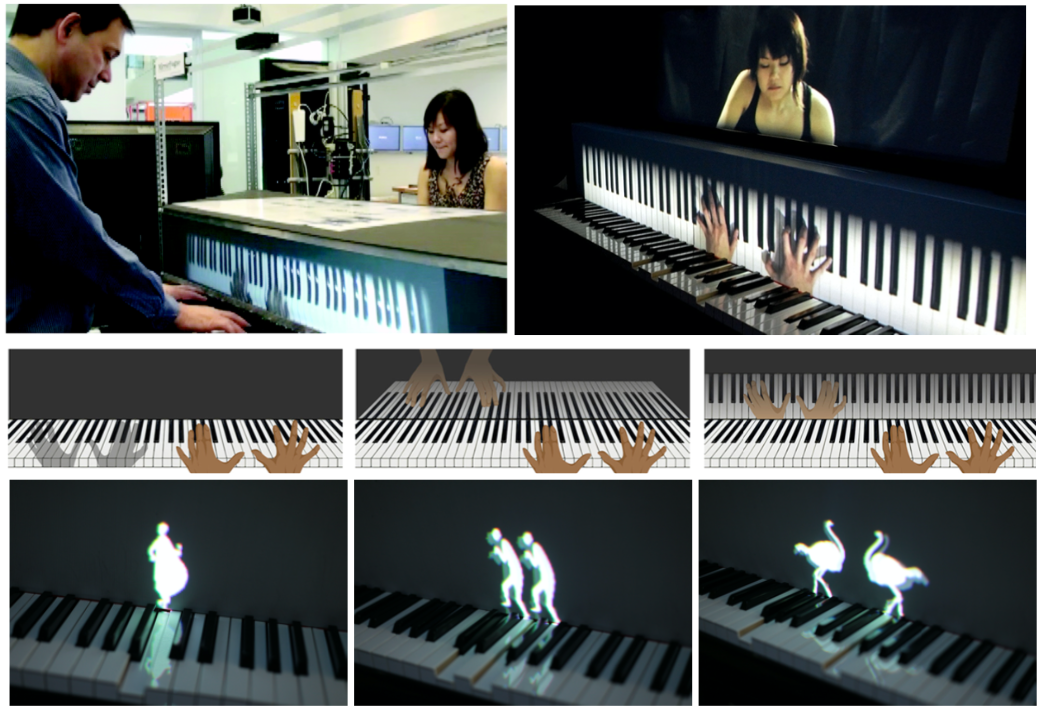
\includegraphics[width=18cm]{figures/xiao.png}
  %  \caption{Agents and tutors in the MirrorFugue series. \textbf{Top left:} MirrorFugue I: piano duet prototype where a tutor sits across the learner. A camera is setup on top of the hands of the tutor. This is fed and viewed into a projection that is seen by the learner positioned just above the keys of the learner. \cite{xiao2010mirrorfugue}. The goal of this prototype to communicate proper hand gestures but with collaboration as the focus. \textbf{Top right:} MirrorFugue III: this prototype \cite{xiao2013mirrorfugue} projects (they used the word \textit{"conjures"} instead of projects) a recorded pianist instead of a live pianist used in \cite{xiao2010mirrorfugue}. In this setup, it focuses on teaching the learner to press the right keys similar to that of an expert pianist as seen in the projection. \textbf{Middle:} The concept photo for the proposed interface done in the work of \cite{xiao2010mirrorfugue}. It introduces the shadow mode, the mirror mode opposite the learner and the mirror mode beside the learner. This explores the different modes on which position and posture of the visualization will fit best in teaching the right finger positioning and timing in pressing.  \textbf{Bottom:} Andante: the latest incremental improvement in the Mirrofugue series, which uses creating and dancing animations as projections instead of a the virtual pianist, as piano roll representations. The movements and steps shown by the animated figures guide the user on the tempo and the right keys to press in the piano. }
 %   \label{fig:xiao}
%\end{figure*}

In augmented piano prototypes, having an augmented reality keyboard or an interactive keyboard has been an obvious choice. These studies served as the test bed for spatial registration, rendering and optimization of graphics in mobile AR. Another addition to augmented piano prototypes is the use of augmented agents and tutors. Only 9 out of 40 prototypes (22\% of the total) had virtual agents and tutors as part of their contribution. These virtual characters, at the time, were computationally-extensive but considered exciting. Some augmented piano prototypes have designed augmented agents and tutors that assist the novice piano learner. The development of agents and tutors would usually have two distinct focus namely (1) designing and rendering agents to appear as human-like or as realistic as possible and (2) designing them to be as intelligent as possible. In the context of augmented piano prototypes, the improved user experience has also been considered more recently. 

The MirrorFugue series \cite{xiao2010mirrorfugue, xiao2011duet, xiao2013mirrorfugue, xiao2014andante} (as seen in Fig \ref{fig:xiao}) features augmented piano prototypes that attempts to address not only the two focus but also introduces a third focus for AR agents and tutors - which is to give pleasant and exciting experiences with an agent. In order to do this, they developed multiple iterations of the augmented piano prototype that considers several use-cases. First, they attempted to gauge collaboration between a learner and a tutor. A regular keyboard is equipped with special cameras and projections that show to the novice, the hand movements of the more experienced user. Second, their work introduced various interfaces (shadow and reflection) and they measured which among these interfaces would best visualize the movement of the tutor in a way that is easiest for the learner. Then, they tested with various modes on how to project these reflections. One mode displayed a shadow hand beside the player. Another mode, had hands reflected from dashboard of the keyboard, giving the player a mirror's view similar to how dancers would follow a choreographer's movements. In the latest version of their prototype, they pivoted the design of their agent from a reflection to using animated agents. Their results led novices on how to play the keyboard by following the movement of these agents. As seen in Fig \ref{fig:xiao} (bottom part), augmented agents that were configured with musical notation (such as tempo, pitch, etc) dance during a performance thereby leading the user on how to play the piano. 

%% no need to sketch this. unless we dont have enough space to consume
%\begin{figure}[t]
  %  \centering
 %   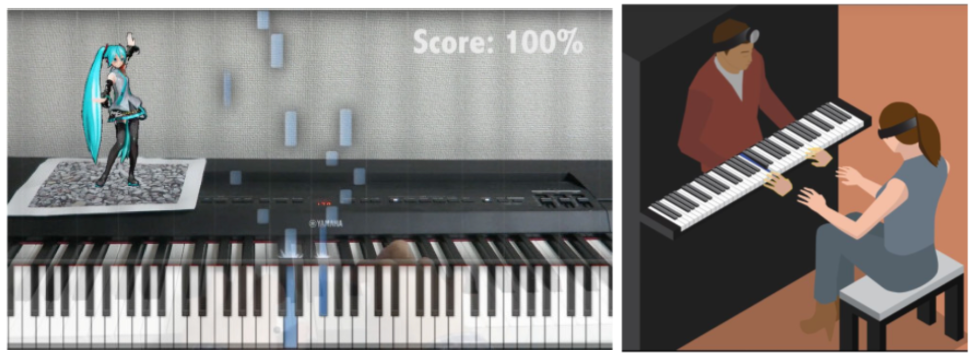
\includegraphics[width=8.5cm]{figures/goodwingerry.png}
  %  \caption{Featured prototypes that use agents and tutors. \textbf{Left:} The work of \cite{goodwin2013key} which was published in 2013. It was still using marker technologies to track an anime-inspired agent. It uses piano roll visualizations which were being displayed when the agent dances. It was also measuring timing and accuracy to gauge the user's performance.  \textbf{Right:} The ADEPT prototype \cite{gerry2019adept} where a user sees and embodies a piano tutor through a virtual agent. Users wear a glove which serves as guide that they can follow. }
 %   \label{fig:goodwingerry}
%\end{figure}

The Augmented Design to Embody a Piano Teacher (ADEPT) \cite{gerry2019adept} provides a first-person audiovisual perspective of the teacher to the tutor. In other works, learners usually follow the guide or walkthrough by a tutor but in this study, they are guided by a tutor that is embodied in their point of view (POV). Learners wear a virtual glove that they see through a head-mounted display and follow the lead of a virtual tutor. This virtual tutor shows an actual person in a separate room, where their hand movements are recorded and projected as an embodiement to the vision of the learner. The work of \cite{goodwin2013key} took entertaining to the next level by using \textit{anime}\textendash inspired agents to teach piano. The agent used marker-technology for tracking and had piano roll visualization as well to guide the user. 

\subsubsection{Piano roll visualizations as substitute for complex notation}
\label{subsec: pianoroll}

%% no need to sketch this unless we need more space to consume 
%\begin{figure}[h]
  %  \centering
  %  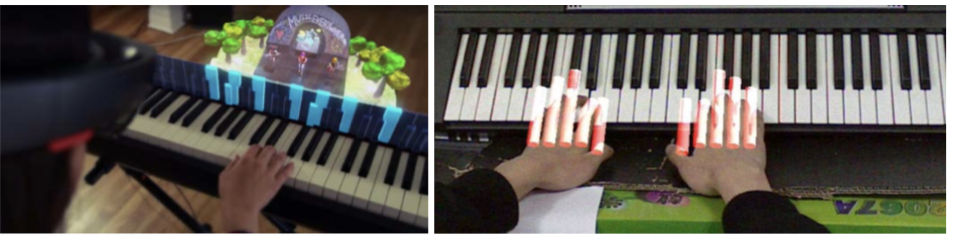
\includegraphics[width=8.5cm]{figures/dashuang.png}
 %   \caption{Stationary piano roll visualizations in head-mounted displays. \textbf{Left:} The augmented piano prototype described in the work of \citet{das2017music}. In this mixed reality setup, users wear a headmounted display where they see piano roll visualizations by the edge of the keyboard thereby guiding the users on what specific keys to press. An agent performer is also seen to entertain the piano player, moving depending on the rhythm provided. \textbf{Right:} The augmented piano prototype described in the work of \citet{huang2011piano}. A user wears a head-mounted display while operating a real piano. The mobile device in the head-mounted display sees the piano and renders graphics on top of the keys, guiding the user on which key to press. The visualizations on both of these studies appear stationary.  }
 %   \label{fig:dashuang}
%\end{figure}
The most cited difficulty in learning how to play the piano is the learning curve introduced by the music sheet notation. This is why a popular approach (26 out of 40 \textendash  which is 67\% of these prototypes)for this problem is to use interactive piano roll visualizations. Piano roll visualizations in AR are music visualizations that novice players can use. They serve as an easier representation to read complex music sheet notation, enabling novice users to quickly learn the piano \cite{walder2016modelling}. In this approach, the learning curve is reduced as novices need not to learn (yet) complex music notation and can focus on proper finger positioning, placement and accuracy. These visualizations usually come in polyphonic form to represent multiple melodies that take place in the same concurrent time segment \cite{ciuha2010visualization}.  Piano rolls have been used as well such for the guitar \cite{biamonte2010musical}, drum \cite{rossignol2015alternate} and many others. It is important to note that piano roll visualizations do not necessarily mean they are visualizations for piano. But rather, they represent a group of visualizations that move and unveil sound information as the visualizations are reveled, similar to the traditional piano roll music box. In general, piano roll visualizations refer to a group of visualizations that behave similarly with movie credits, rhythm games and many others. 

Piano roll visualizations are designed to guide users on which key to press at the right time. This gives the spatiotemporal component (\textit{spatio} - position in multidimensional space, and \textit{temporal} - movement with consideration of time as the major element) depending on the platform and environment where they are implemented. The graphics are usually overlaid near or on top of the piano keys moving (either be downwards or sideways depending on the target) towards the button that the user should press. 

These visualizations used for AR prototypes have appeared in different forms. augmented piano prototypes that are mobile-based or that may need a head-mounted display would render their piano roll visualizations to show as if they were on top of a real piano. On most cases, these visualizations appear on top of the piano keys seen through the camera of the mobile device (see Fig \ref{fig:dashuang}). Some of them are stationary and do not move, serving only as visual stimuli waiting for the user to input and press the key below them. Some visualizations are non-stationary, actively moving towards the keys to press, based on a given song's tempo (see Fig \ref{fig:caitrujano} Left ). Some of them have been found on AR prototypes where they display piano roll visualizations outside of the mobile device or head-mounted display. These augmented piano prototypes have been designed to display visualizations in wider spaces through a 3D projector or specialized cameras like the Kinect. These moving visualizations denote extra meaning, sometimes sending additional feedback to the users. They may appear in a given color (usually blue or any neutral color) to denote that they should be pressed next (or soon). Then they appear in a different color to denote the success of the pressing (green for good timing, yellow for somewhat delayed timing and red for missed or wrong key pressed) (see Fig \ref{fig:caitrujano} Right and Fig \ref{fig:projectors}). 

\todoj{sketch caitrujano !! }
%\begin{figure}[t]
 %   \centering
  %  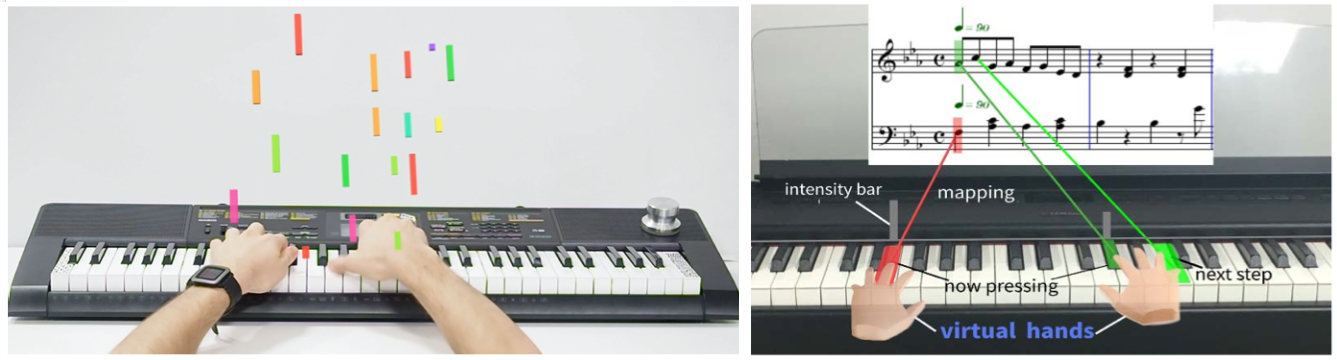
\includegraphics[width=8.5cm]{figures/caitrujano.png}
  %  \caption{Moving piano roll visualizations in head-mounted displays. \textbf{Left}: The piano roll visualizations in the prototype by  \cite{trujano2018arpiano} uses a head-mounted display and uses a minimalist interface. Key visualizations appear in random colors and seem to come out of nowhere. As the graphics draw closer to their respective keys, they slowly fade. No feedback exists to show whether the keys pressed are correct or not.  \textbf{Right}: Preview of the architecture of the prototype described in \cite{cai2019design}. The prototype uses \textit{"intensity bars"} as piano roll visualizations that appear in two colors: red (now pressing) and green (next to press). These intensity bars are mapped directly with their equivalent notes as seen in the music sheet. Virtual hands are displayed as well in helping the user position their hands. }
 %   \label{fig:caitrujano}
%\end{figure}
There are also specific types of piano roll visualizations that are non-stationary. These visualizations appear to move within a specific time frame giving the user the notion of temporality (see Fig \ref{fig:caitrujano}). As these visualizations move, they teach two things to the user: (1) knowing the right key to press at the right time and (2) mapping the complex music notation and their equivalent key press. Some of these piano roll visualizations have also been introduced in a gamified mode \cite{Weing:2013:PEI:2494091.2494113} which researchers believe allowed learners to learn faster or easier. More on these learning modes will be discussed in subsection \ref{subsec: learn}. 

\subsubsection{Newer techniques in assessing and evaluating augmented piano learners}
\label{subsec: eval}
Of the 40 papers included in this review, only 18 (45\% as seen in Table \ref{tab:overview}) have performed user studies on the system  as part of their contribution. These user studies evaluated certain factors such as ease of use, satisfaction, immersion, motivation and performance among many others. We believe that through the development of augmented piano prototypes, techniques and methods on evaluating these factors have changed and improved as well. Following the data gathering techniques described in subsection \ref{subsec: gathering}, we reviewed these papers and analyzed how they did their user studies. We looked at their sample size, the type of their participants, the type of treatment, the metrics or constructs they measured and the tools/instruments they used to measure these metrics. In our review, we observed a shift of focus in treatment and metrics in the same way the shift in focus for visualizations and agents/tutors have taken place. 
What separates HCI research from other disciplines is it properly gauge the impact of the prototypes, systems into their human users. Specific human factors and affordances are usually discovered as these user studies are done. We begin looking at these evaluation techniques introduced with the participants involved and their respective size. The number of participants involved in these studies ranged from 1 to 74, with a median sample size of 8.5 (see Table \ref{tab: us-all}). These involved a combination of expert and novice users, people with or without background in using AR apps and tools. There was even one study who involved patients with disabilities as part of their respondents \cite{correa2009computer}. These studies considered various study designs from between-subject, within-subject, with or without control groups and many others. Since there are other contribution categories introduced by these papers, they have different focus in terms of treatment (see Table \ref{tab: us-all}). These were also depending on the year the studies were published from (either between 2005-2010, 2011-2015 or 2016-2020). Earlier studies tend to measure usability in consideration accuracy of spatial registration (such as marker detection). Newer studies focused on measuring activities where users are more free (or have more flexibility) to play around with the tool. These studies have their users do task-oriented use cases (such as playing major or minor chords \cite{nugraha2014pemanfaatan, xiao2010mirrorfugue}, play a specific song or piano piece \cite{chow2013music, sandnes2019enhanced,pan2018pilot} or simply practice the piano on their own for a specific amount of time \cite{weing2013piano, raymaekers2014game}). In some studies, adding familiar and entertaining elements have allowed experiments that focused on gamification, and the ability of the users to complete quests as an alternative approach to measuring performance and learning. 

\begin{table*}[t]
\caption{List of studies with user evaluation (labelled as \textit{US} as seen from Table \ref{tab:overview}). This table provides an overview of their treatments, metrics, constructs and tools used. \textit{Treatment Legend}: \textit{ex}= free usage and exploration modes; \textit{md}= marker detection; \textit{ob}= observation of prototype usage; \textit{pc}= play piano chords on the piano;  \textit{pl}= play a piece in the piano; \textit{pr}= practice the piano; \textit{qu}= complete quest in a game or gamified interface.  \textit{Metrics Legend}:   \textit{At}= attractiveness; \textit{CL}= cognitive load; \textit{FI}= accuracy of finger information; \textit{Im}= level and quality of immersiveness; \textit{Mo}= level of user motivation; \textit{No}= accuracy of notation; \textit{Op}= functional check of the different features of the prototype; \textit{Sa}= satisfaction rating of the prototype; \textit{Sk}= improvement in skill; \textit{Us}= ease of use and usability; \textit{TI}= time interval and usage of the system; \textit{Sc}= scoring (for gamified prototypes). \textbf{Tools Legend}: \textit{OEQ}= open ended questionnaires; \textit{QUE}= used a peer-reviewed questionnaire/instrument; \textit{PSP}= player scoring plug-ins; \textit{REC}= observations from recordings; \textit{SMQ}= self made questionnaire; \textit{SSI}= semi structured interviews; \textit{TTM}= time tracking mechanisms. }
\label{tab: us-all}
%\resizebox{\textwidth}{!}{%
\small\begin{tabularx}{\textwidth}{lclllllX} \toprule
\textbf{Ref.}                           & \textbf{Size} (\textit{n})    & \textbf{Treatment}    & \textbf{Metrics or constructs}    & \textbf{Tools} & \textbf{Notes }\\ \midrule
%P1 \cite{huang2011piano}              & 2011 &        & a                         & a                             & a                    \\
\cite{nugraha2014pemanfaatan}        & 8            & md, pc      & At, Op, Us             & SMQ                   & \\ \hline
\cite{chow2013music}                 & 7            & pl          & Sa, Us                 & OEQ                   & \\ \hline
\cite{weing2013piano}                & 5            & ex, pr      & CL, FI, No, Sa         & SMQ                   & \\ \hline
\cite{kerdvibulvech2017innovative}   & 1            & pl          & Sc, TI                 & TTM                   & \\ \hline
\cite{schmalstieg2007experiences}    & 6            & pl, qu      & Sa, TI                 & PSP, SSI, TTM         & \\ \hline 
\cite{correa2009computer}            & 1            & ex, qu      & Op, Us*                & REC, TTM              & \textit{*patient motor effects} \\ \hline 
\cite{takegawa2012piano}             & 9            & pl, pr      & FI, No, Sc, TI         & PSP, SSI, TTM         &   \\ \hline
\cite{xiao2010mirrorfugue}           & 5            & pc, pl*     & Im, Op                 & PSP, REC, SSI, TTM    & \textit{*improvise a piece}\\ \hline
\cite{xiao2013mirrorfugue}           & 15           & ob          & Im, Op, Us             & SMQ, SSI              &  \\ \hline
\cite{li2018application}             & 17           & ex, ob      & Mo, Op                 & QUE*                  & \textit{*instrument from }\cite{zhang2000relationship}    \\ \hline
\cite{leonard2013virtual}            & 20           & ex, pr      & Op, Sa, Sk             & OEQ, TTM              &    \\ \hline
\cite{raymaekers2014game}            & \textendash* & ex, pl, pr  & At, Sa, Us             & OEQ, REC              & \textit{*open demo UT} \\ \hline
\cite{rogers2014piano}               & 74*          & pc, pl, pr  & At, CL, Sa, Sk, Us, TI & QUE$^\dagger$            & *$n_{1}$=56, \begin{math}n_{2}\end{math}=18, $^\dagger$\cite{ekstrom1976manual, klepsch2012subjective, hassenzahl2003attrakdiff, wrigley2013ecological}\\ \hline
\cite{sun2018mr}                     & 20           & ex, pc, pl  & Sc, Sk, Us, TI         & PSP, TTM              &   \\ \hline
\cite{molloy2019mixed}               & 23           & pl          & At, Im, Mo, Us         & OEQ, QUE*, SSI        & *SUS\cite{lewis2009factor}\\ \hline
\cite{pan2018pilot}                  & 13           & pl, pr      & Sc, Sk                 & OEQ, PSP, SMQ, SSI    &  \\ \hline
\cite{kim2014ar}                     & \textendash* & ex, md      & FI, Op                 & REC                   & \textit{*n not reported}  \\ \hline
\cite{xiao2011duet}                  & 3            & ex, ob      & Im, Us                 & SSI                   &   \\ \hline 
\cite{ogata2017keyboard}             & 3            & ex, pl      & Op, Sa                 & SMQ                   &   \\ \hline 
\cite{mcpherson2013space}            & 8            & pl, md      & FI, No, Op             & PSP, TTM              &   \\ \hline 
\cite{mcpherson2011multidimensional} & 30*           & ex, pl      & FI, No, Op, Us, TI     & REC, TTM              & *3 tests with 10 $n$ each  \\ \hline 
\cite{granieri2019reach}             & -*           & ex          & Im                     & REC                   & \textit{*open demo UT, n not reported}  \\ \hline 
\cite{karolus2020hit}                & 12           & ex, pl      & At, CL, Op, Sa, TI     & OEQ, QUE*, TTM                  &  *NASA TLX\cite{hart1988development}, CSI\cite{carroll2009creativity}, HEMA\cite{huta2010pursuing} \\ \midrule 
                                   & \textit{med.}=8.5 & \textit{\={x}}=14   &                   &                       & \\ \bottomrule
\end{tabularx}%
\end{table*}

The introduction of task-oriented use-cases in evaluating usability in these augmented piano prototypes led to the use of newer metrics and/or constructs that properly-describe them. Metrics that used to be difficult to measure are now defined in these newer studies thanks to recent innovations as well. Earlier AR prototypes focused on measuring attractiveness and function. Since AR technologies allow a person to be immersed between virtual and actual reality \cite{milgram1995augmented}, metrics that define immersion (how a person is immersed in an AR artifact) have been used as well. As users get immersed, this leads to significant impacts in cognitive load and their state of being overwhelmed. Cognitive load, and other affect measures such as user motivation give additional insight on the usability of these AR prototypes as well. These constructs allowed augmented piano prototype researchers to finally look at the core important factor which is piano learning without having to think of specific implementation issues (such as spatial registration, object tracking, etc). In order to fully understand and accurately-assess piano learning, additional metrics have also been considered such as time interval, key-press accuracy, mastery of music notation, scoring based on hit-miss accuracy and other skill improvement measures. There were other specific metrics or constructs observed in these studies that are considered unique or not well-investigated such as the impact of AR on motor effects of patients with cerebral palsy, how the interface supports team-play and collaboration among multiple users and many others. 

Along with the development of metrics or that assess piano skill learning, are the introduction of tools and instruments that support these constructs. In these user studies, observations, interviews (both pre and post) allowed augmented piano prototype developers to understand their users and the insights they discover deeper. Some studies consider a mixed-method design where they employ plug-ins and programs that measure specific indicators (quantitative - such as tracking of key-press, recording of time intervals between practices, assigning points in gamified modes; qualitative - such as think out aloud protocol, facial expressions observed by coders and annotators, etc). Studies that measured cognitive load have used advanced sensors such as galvanic skin response (GSR) and electrocardiogram (ECG). It is interesting to note that a great number of the studies reviewed in this paper have used their own self-made questionnaires (see label \textbf{SMQ} in Table \ref{tab: us-all}). The use of semi-structured interviews along with these self made questionnaires have been a popular choice for their study design. Only a few studies have used peer-reviewed and established questionnaires and instruments (such as Attrakdiff \cite{hassenzahl2003attrakdiff} and SUS \cite{lewis2009factor})  in their study design. Some articles reviewed did user studies in informal settings where participant criteria and sampling were not clearly-defined or were not restricted to a specific demographic type. 

Other evaluation methods and tools demonstrated their specific advantages and disadvantages depending on how the studies were done. For example, semi-structured interviews and observations were more helpful in understanding usability factors in using augmented piano prototypes. Expert reviews played a crucial role in measuring learning and skill improvement. Having control groups in between user studies of these augmented piano prototypes allowed researchers to understand if there are actual improvements introduced by these prototypes (measured by ANOVA, significant difference and other statistical tools) as compared to the traditional setup of using the piano. 



%\subsection{Hand tracking}
%\label{subsec: ht}
%Im still studying HT. prolly last that I will write


%\begin{figure}[t]
 %   \centering
 %%   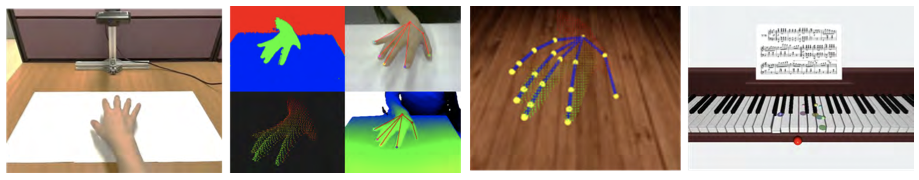
\includegraphics[width=8.5cm]{figures/lianghandtrack.png}
 %   \caption{Different forms of hand tracking for the piano done in the work of \cite{liang2016barehanded}. It considers lighting and how a hand is placed on top of a white background (\textbf{first}), segments the hand based on image processing techniques (\textbf{second}), identifies joints and action points of the fingers in the (\textbf{third}) and its positioning in an augmented piano (\textbf{fourth}). }
 %   \label{fig:lianghandtrack}
%\end{figure}
Text here. 

\subsubsection{Learning modes for independent and sustained novice practice}
\label{subsec: learn}

\todoj{sketch projectors.png !!}
%\begin{figure*}[t]
 %   \centering
 %   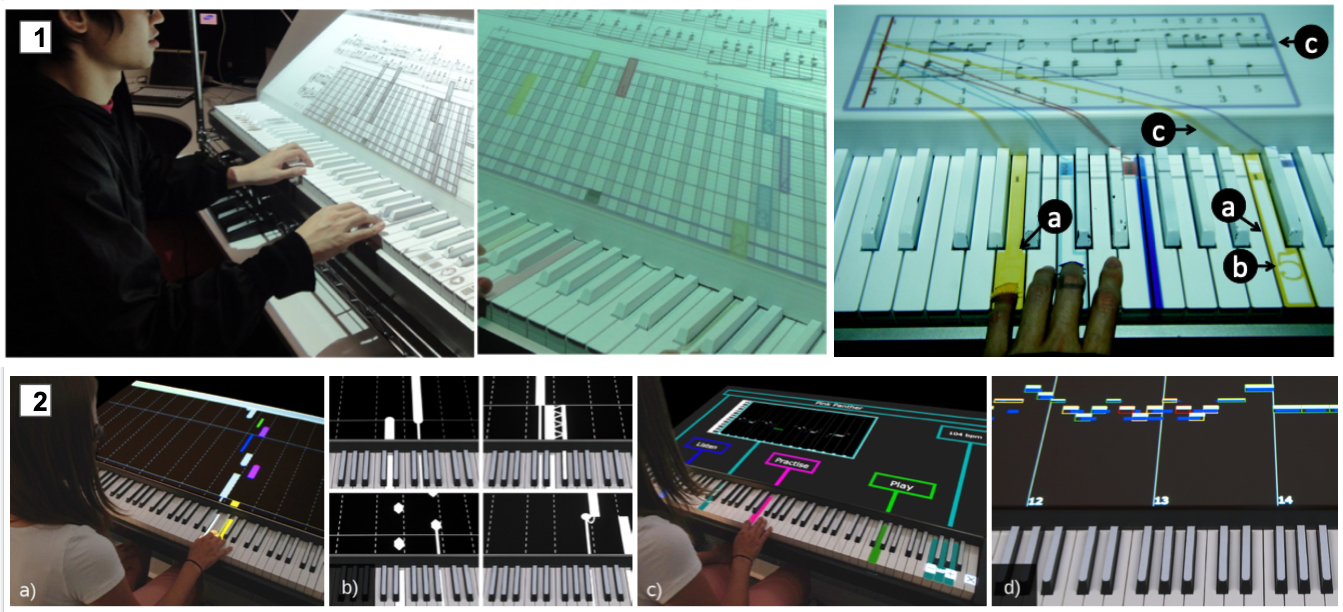
\includegraphics[width=18cm]{figures/projectors.png}
 %   \caption{Projector-based visualizations and their learning modes.  \textbf{\#1}: The prototype by \cite{takegawa2012piano}. It utilizes a projector that displays the piano roll visualizations on top of an actual piano. The black keys in the piano have been recoloured to white. Specific colored visualizations appear on top of each keys guiding the user on what and when to press. A music notation sheet which is drawn with colored lines are mapped to the piano roll notations that overlay the piano keys. In their approach, the music sheet is transformed into lines, which point to piano roll visualizations that are overlaid on top of the keys that the users can press. \textbf{\#2}: The prototype in \cite{rogers2014piano} which uses a similar projection technique with that of Takegawa et al. However, their prototype introduces learning modes which change how the piano roll visualizations are displayed. Depending on the mode, the piano roll can move downwards similar to that of rhythm games, or like building blocks that are read from left to right. }
 %   \label{fig:projectors}
%\end{figure*}

One main concern as to why we build augmented piano prototypes is because we want to help piano learners in the learning process. Developers have created augmented piano prototypes in a way that is considers the context of learning, skill improvement for piano novices. This was done by introducing various learning modes which began to emerge in the latter era. Of the 18 articles (as described in subsection \ref{subsec: eval}), only 7 (17\% of all the articles covered, 38\% of US-studies) incorporated learning modes as part of their contribution. Another 5 articles (who did not have a user study as part of the contribution) introduced learning modes as well as part of their prototype - but these were not evaluated in a user study. A Practice mode has been a common part of these learning modes. A self-reflection learning mode has also been introduced by a few studies \cite{gerry2019adept, xu20195, xiao2013mirrorfugue}. In this mode, users of the augmented piano prototypes can watch and view their own performance - either in real time or after an experiment treatment. We believe that this feature is draws inspiration from the theory of \citet{zimmerman2009self} on how self-reflection promotes self-regulated learning as seen on some various learning experiments \cite{deja2016discovering,lyons2011monitoring}. Since augmented piano prototypes were developed as an alternative learning environment for piano learning especially when a tutor is absent or when learning can take place on its own, a learning mode such as self-reflection definitely supports this process. 

Aside from self-regulation and self-reflection theory, social learning theory emphasizes four distinct steps in learning namely attention, retention, reproduction and motivation \cite{bandura1977social}. In \textit{attention}, a piano learner observes a process. During \textit{retention}, the piano learner performs activities where they try to remember what they have observed (from the previous step). The \textit{reproduction} then follows this where they perform activities that they have observed. This learning process becomes sustainable that it leads to medium to long-term improvement through the \textit{motivation} step. Here, reinforcement (could be positive or negative) ensures that the novice can continuously practice and learn the piano. The prototype described in the work of \citet{weing2013piano} and \citet{rogers2014piano} supports social learning theory through their design of their learning modes. 

A \textit{listen (attention)} mode allows novices to observe and listen in a song that is visualized in their augmented piano prototype. They considered this mode based on inputs with experts involved in their study. The \textit{practice (retention)} provides novice players a different form of piano roll visualization (as seen in Fig \ref{fig:projectors}). They believe that retention is maintained by showing users of their augmented piano prototype the correct way of playing the keys and allowing them to perform them without haste. In this learning mode, feedback in the form of visualizations, brightly highlights the correct keys and the wrongly-pressed keys. Lastly, in their \textit{play (reproduction and motivation)} mode, users of the augmented piano prototype can receive additional feedback on their performance. They can play a specific song or piano piece \textit{(reproduction)} following a form of piano roll visualization different from practice mode. As users play in this mode, they receive live feedback on their key press. Similar to rhythm games, they also get to see a summary of their performance through a progress bar. With the help of player scoring plug-ins (PSP) and time-tracking mechanims (TTM) (as seen in Table \ref{tab: us-all}), an additional layer of information is shown about their performance. Not only do they see correct or mis-pressed keys, expected notes (missed keys), incorrect duration are also displayed. By self-reflection and seeing an overview of their performance, piano learners are expected to reflect on their progress both at an abstract and low level of detail, which in turn provides \textit{motivation}. Other modes of interaction have also been introduced to aid learning and other piano-related activities. Learning with a partner \cite{xiao2011duet}, performing with a group \cite{gerry2019adept} and learning with a group \cite{cai2019designa}.

%no need to sketch this unless we have more space to consume 
%\begin{figure}[t]
 %   \centering
 %   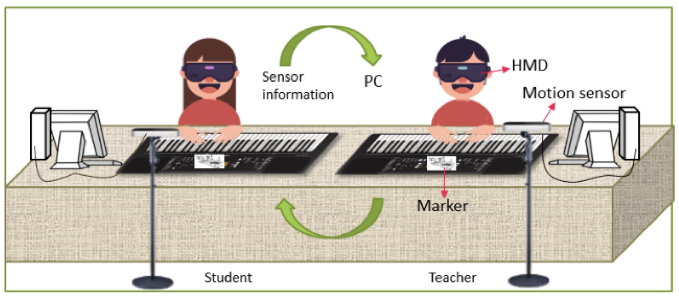
\includegraphics[width=8.5cm]{figures/caigroup.png}
 %   \caption{Multi-user collaboration. In the work described in \cite{cai2019designb} a setup has been designed where at least two users equipped with head-mounted displays can co-perform a musical piece in the augmented piano prototype. They do this by pressing keys following the piano roll visualizations that have have to be pressed and completed by both users. It can be used on two modes, a competitive mode and a collaborative mode where in the former they aim to get a score higher than the other and in the latter, they try to cooperate and work together on a single piano piece.}
 %   \label{fig:caigroup}
%\end{figure}

\todos{Add more here - a summary - outlook}




\subsection{Learner-based themes}
%\label{sec: strat}
From these trends and technological innovations, we were able to draw different themes that we believe have inspired these contributions. In the context of learning, we believe that these themes 

\subsubsection{Ensuring correct finger positioning for novice learners}
\todoj{build discussion here}
\subsubsection{Representing complex sheet notation with augmented visualizations}
\todoj{build discussion here}
\subsubsection{Encouraging self-regulated learners to continuously practice}
\todoj{build discussion here}
\subsubsection{Improving performance of advanced players through improvisation}
\todoj{build discussion here}
\subsubsection{Others}
\todoj{build discussion here}
\subsubsection{Portability}
\subsubsection{Collaboration}

\subsection{Other findings}

\begin{table}[t]
\centering
\caption{Venues where augmented pianos have been published}
\label{tab:venues}
\begin{tabular}{lrr}
%\hline
Venue             & Papers total & \%    \\ \hline \hline
\textbf{CHI}      & 6           & 9.8   \\
\textbf{CHI PLAY} & 1           & 1.6   \\
\textbf{ISMAR}    & 2           & 3.3   \\
\textbf{NIME}     & 11          & 18.0  \\
\textbf{other}    & 41          & 67.2  \\ \hline
total             & 61          & 100.0 \\ 
\end{tabular}
\end{table}

\todoj{paper selection strategy overview}
\todoj{citation graph with colors}
 
\section{Discussion and Future Directions}
%%jordan: from these themes: you identify where are the areas on understand/tracking user progress, managing cognitive load then thish ow you can introduce your future directions
\subsection{Learner Personalisation}
\subsection{Understanding user motion }
\todoj{did any of the works discuss understanding user motion? or their progress? or managing their overload? did }
Have a discussion here Jordan. how does this connect with piano learning? 
Where is spatiotemporal pointing?
can any of these consider proficiency aware systems? 
\label{sec: discuss}
%gaps in modelling? position near your thesis

%text here



%%
%% The next two lines define the bibliography style to be used, and
%% the bibliography file.
\bibliographystyle{ACM-Reference-Format}
\balance
\bibliography{sample-base}

%%
%\nocite{*}
%% If your work has an appendix, this is the place to put it.
%\appendix
\end{document}
\endinput
%%
%% End of file `sample-manuscript.tex'.
